\documentclass{standalone}
\usepackage{tikz}
\usetikzlibrary{patterns, positioning}


\begin{document}
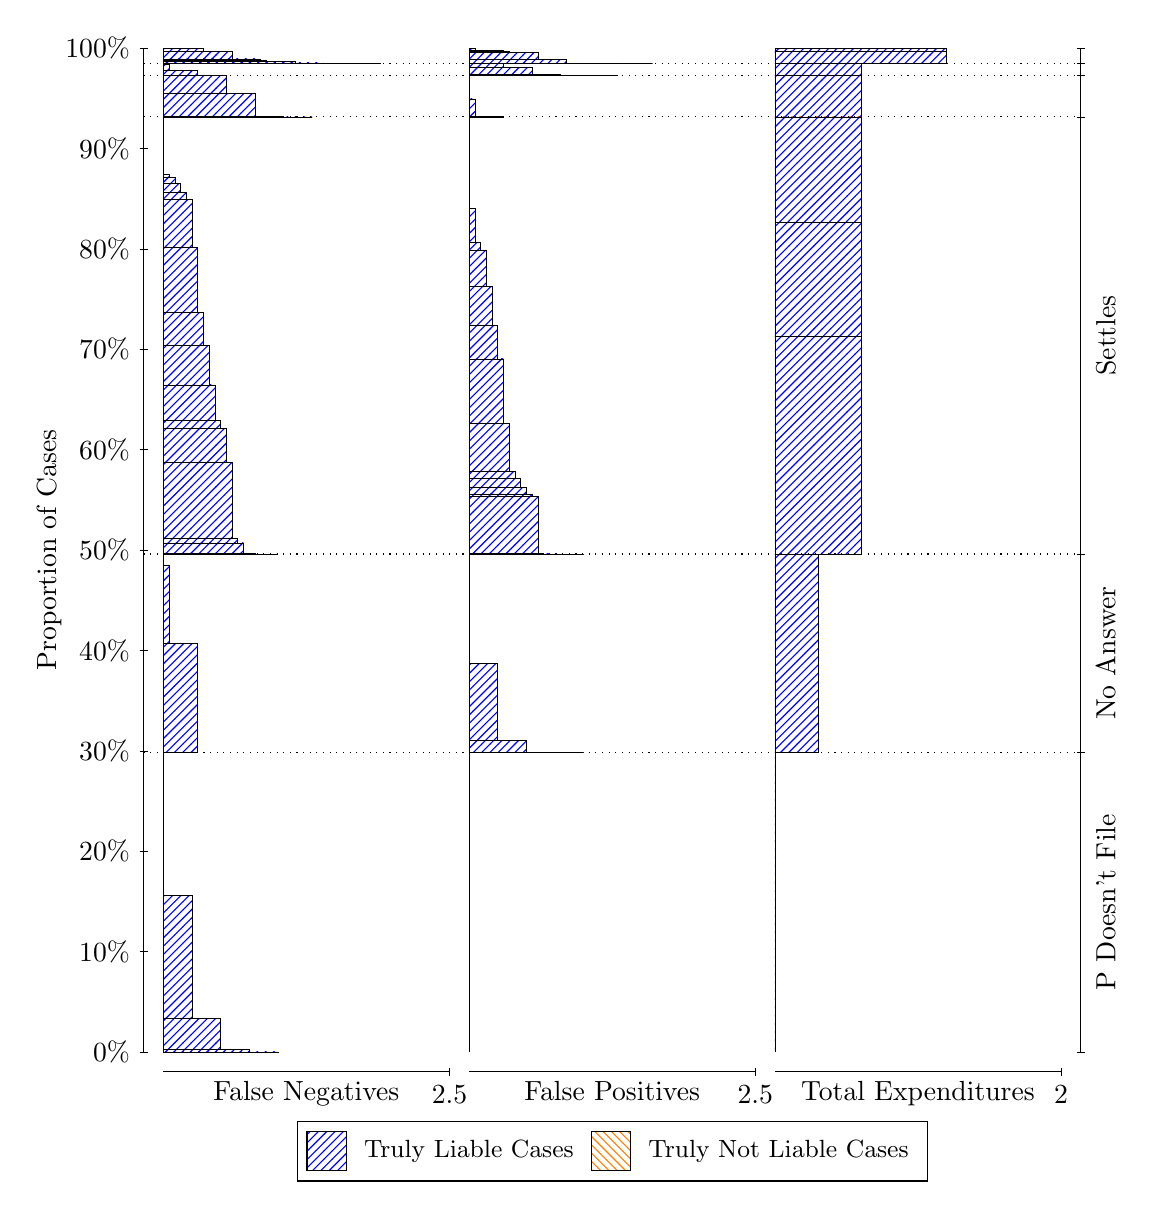
\begin{tikzpicture}
\draw[black, very thin] (1.5,1.75) -- (1.5,14.5);
\node[rotate=90, text=black, anchor=center] at (0.3, 8.125) {Proportion of Cases};
\draw[black, very thin] (1.45,1.75) -- (1.55,1.75);
\node[text=black, anchor=east] at (1.45, 1.75) {0\%};
\draw[black, very thin] (1.45,3.025) -- (1.55,3.025);
\node[text=black, anchor=east] at (1.45, 3.025) {10\%};
\draw[black, very thin] (1.45,4.3) -- (1.55,4.3);
\node[text=black, anchor=east] at (1.45, 4.3) {20\%};
\draw[black, very thin] (1.45,5.575) -- (1.55,5.575);
\node[text=black, anchor=east] at (1.45, 5.575) {30\%};
\draw[black, very thin] (1.45,6.85) -- (1.55,6.85);
\node[text=black, anchor=east] at (1.45, 6.85) {40\%};
\draw[black, very thin] (1.45,8.125) -- (1.55,8.125);
\node[text=black, anchor=east] at (1.45, 8.125) {50\%};
\draw[black, very thin] (1.45,9.4) -- (1.55,9.4);
\node[text=black, anchor=east] at (1.45, 9.4) {60\%};
\draw[black, very thin] (1.45,10.675) -- (1.55,10.675);
\node[text=black, anchor=east] at (1.45, 10.675) {70\%};
\draw[black, very thin] (1.45,11.95) -- (1.55,11.95);
\node[text=black, anchor=east] at (1.45, 11.95) {80\%};
\draw[black, very thin] (1.45,13.225) -- (1.55,13.225);
\node[text=black, anchor=east] at (1.45, 13.225) {90\%};
\draw[black, very thin] (1.45,14.5) -- (1.55,14.5);
\node[text=black, anchor=east] at (1.45, 14.5) {100\%};

\draw[black, very thin] (13.4,1.75) -- (13.4,14.5);
\draw[black, very thin] (13.35,1.75) -- (13.45,1.75);
\node[anchor=west] at (13.35, 1.75) {};
\draw[black, very thin] (13.35,5.5544) -- (13.45,5.5544);
\node[anchor=west] at (13.35, 5.5544) {};
\draw[black, very thin] (13.35,8.0739) -- (13.45,8.0739);
\node[anchor=west] at (13.35, 8.0739) {};
\draw[black, very thin] (13.35,13.625) -- (13.45,13.625);
\node[anchor=west] at (13.35, 13.625) {};
\draw[black, very thin] (13.35,14.156) -- (13.45,14.156);
\node[anchor=west] at (13.35, 14.156) {};
\draw[black, very thin] (13.35,14.306) -- (13.45,14.306);
\node[anchor=west] at (13.35, 14.306) {};
\draw[black, very thin] (13.35,14.5) -- (13.45,14.5);
\node[anchor=west] at (13.35, 14.5) {};

\draw[black, very thin, pattern color=blue, pattern=north east lines] (1.75,1.75) rectangle (3.2033,1.7503);
\draw[black, very thin, pattern color=blue, pattern=north east lines] (1.75,1.7503) rectangle (2.84,1.7783);
\draw[black, very thin, pattern color=blue, pattern=north east lines] (1.75,1.7783) rectangle (2.4767,2.178);
\draw[black, very thin, pattern color=blue, pattern=north east lines] (1.75,2.178) rectangle (2.1133,3.7356);
\draw[black, very thin, pattern color=orange, pattern=north west lines] (1.75,3.7356) rectangle (1.75,3.7356);
\draw[black, very thin, pattern color=blue, pattern=north east lines] (1.75,3.7356) rectangle (1.75,5.5544);
\draw[black, very thin, pattern color=blue, pattern=north east lines] (1.75,5.5544) rectangle (2.186,6.943);
\draw[black, very thin, pattern color=blue, pattern=north east lines] (1.75,6.943) rectangle (1.8227,7.9257);
\draw[black, very thin, pattern color=orange, pattern=north west lines] (1.75,7.9257) rectangle (1.75,7.9257);
\draw[black, very thin, pattern color=blue, pattern=north east lines] (1.75,7.9257) rectangle (1.75,8.0739);
\draw[black, very thin, pattern color=blue, pattern=north east lines] (1.75,8.0739) rectangle (3.2033,8.0739);
\draw[black, very thin, pattern color=blue, pattern=north east lines] (1.75,8.0739) rectangle (3.058,8.0741);
\draw[black, very thin, pattern color=blue, pattern=north east lines] (1.75,8.0741) rectangle (2.9127,8.0862);
\draw[black, very thin, pattern color=blue, pattern=north east lines] (1.75,8.0862) rectangle (2.84,8.0868);
\draw[black, very thin, pattern color=blue, pattern=north east lines] (1.75,8.0868) rectangle (2.7673,8.2161);
\draw[black, very thin, pattern color=blue, pattern=north east lines] (1.75,8.2161) rectangle (2.6947,8.2744);
\draw[black, very thin, pattern color=blue, pattern=north east lines] (1.75,8.2744) rectangle (2.622,9.2357);
\draw[black, very thin, pattern color=blue, pattern=north east lines] (1.75,9.2357) rectangle (2.5493,9.6653);
\draw[black, very thin, pattern color=blue, pattern=north east lines] (1.75,9.6653) rectangle (2.4767,9.7711);
\draw[black, very thin, pattern color=blue, pattern=north east lines] (1.75,9.7711) rectangle (2.404,10.223);
\draw[black, very thin, pattern color=blue, pattern=north east lines] (1.75,10.223) rectangle (2.3313,10.72);
\draw[black, very thin, pattern color=blue, pattern=north east lines] (1.75,10.72) rectangle (2.2587,11.146);
\draw[black, very thin, pattern color=blue, pattern=north east lines] (1.75,11.146) rectangle (2.186,11.967);
\draw[black, very thin, pattern color=blue, pattern=north east lines] (1.75,11.967) rectangle (2.1133,12.58);
\draw[black, very thin, pattern color=blue, pattern=north east lines] (1.75,12.58) rectangle (2.0407,12.665);
\draw[black, very thin, pattern color=blue, pattern=north east lines] (1.75,12.665) rectangle (1.968,12.781);
\draw[black, very thin, pattern color=blue, pattern=north east lines] (1.75,12.781) rectangle (1.8953,12.862);
\draw[black, very thin, pattern color=blue, pattern=north east lines] (1.75,12.862) rectangle (1.8227,12.893);
\draw[black, very thin, pattern color=orange, pattern=north west lines] (1.75,12.893) rectangle (1.75,12.893);
\draw[black, very thin, pattern color=blue, pattern=north east lines] (1.75,12.893) rectangle (1.75,13.625);
\draw[black, very thin, pattern color=blue, pattern=north east lines] (1.75,13.625) rectangle (3.6393,13.625);
\draw[black, very thin, pattern color=blue, pattern=north east lines] (1.75,13.625) rectangle (3.276,13.631);
\draw[black, very thin, pattern color=blue, pattern=north east lines] (1.75,13.631) rectangle (2.9127,13.928);
\draw[black, very thin, pattern color=blue, pattern=north east lines] (1.75,13.928) rectangle (2.5493,14.153);
\draw[black, very thin, pattern color=blue, pattern=north east lines] (1.75,14.153) rectangle (2.186,14.156);
\draw[black, very thin, pattern color=orange, pattern=north west lines] (1.75,14.156) rectangle (1.75,14.156);
\draw[black, very thin, pattern color=blue, pattern=north east lines] (1.75,14.156) rectangle (2.186,14.212);
\draw[black, very thin, pattern color=blue, pattern=north east lines] (1.75,14.212) rectangle (1.8227,14.298);
\draw[black, very thin, pattern color=orange, pattern=north west lines] (1.75,14.298) rectangle (1.75,14.298);
\draw[black, very thin, pattern color=blue, pattern=north east lines] (1.75,14.298) rectangle (1.75,14.306);
\draw[black, very thin, pattern color=blue, pattern=north east lines] (1.75,14.306) rectangle (4.5113,14.306);
\draw[black, very thin, pattern color=blue, pattern=north east lines] (1.75,14.306) rectangle (4.148,14.306);
\draw[black, very thin, pattern color=blue, pattern=north east lines] (1.75,14.306) rectangle (3.7847,14.31);
\draw[black, very thin, pattern color=blue, pattern=north east lines] (1.75,14.31) rectangle (3.712,14.31);
\draw[black, very thin, pattern color=blue, pattern=north east lines] (1.75,14.31) rectangle (3.4213,14.335);
\draw[black, very thin, pattern color=blue, pattern=north east lines] (1.75,14.335) rectangle (3.3487,14.335);
\draw[black, very thin, pattern color=blue, pattern=north east lines] (1.75,14.335) rectangle (3.058,14.342);
\draw[black, very thin, pattern color=blue, pattern=north east lines] (1.75,14.342) rectangle (2.9853,14.362);
\draw[black, very thin, pattern color=blue, pattern=north east lines] (1.75,14.362) rectangle (2.6947,14.362);
\draw[black, very thin, pattern color=blue, pattern=north east lines] (1.75,14.362) rectangle (2.622,14.453);
\draw[black, very thin, pattern color=blue, pattern=north east lines] (1.75,14.453) rectangle (2.3313,14.453);
\draw[black, very thin, pattern color=blue, pattern=north east lines] (1.75,14.453) rectangle (2.2587,14.497);
\draw[black, very thin, pattern color=blue, pattern=north east lines] (1.75,14.497) rectangle (1.8953,14.5);
\draw[black, very thin, pattern color=orange, pattern=north west lines] (1.75,14.5) rectangle (1.75,14.5);
\draw[black, very thin, pattern color=blue, pattern=north east lines] (1.75,14.5) rectangle (1.75,14.5);
\draw[black, very thin, pattern color=orange, pattern=north west lines] (5.6333,1.75) rectangle (5.6333,1.75);
\draw[black, very thin, pattern color=blue, pattern=north east lines] (5.6333,1.75) rectangle (5.6333,5.5544);
\draw[black, very thin, pattern color=orange, pattern=north west lines] (5.6333,5.5544) rectangle (7.0867,5.5544);
\draw[black, very thin, pattern color=blue, pattern=north east lines] (5.6333,5.5544) rectangle (7.0867,5.5544);
\draw[black, very thin, pattern color=blue, pattern=north east lines] (5.6333,5.5544) rectangle (6.7233,5.5546);
\draw[black, very thin, pattern color=blue, pattern=north east lines] (5.6333,5.5546) rectangle (6.36,5.7027);
\draw[black, very thin, pattern color=blue, pattern=north east lines] (5.6333,5.7027) rectangle (5.9967,6.6853);
\draw[black, very thin, pattern color=blue, pattern=north east lines] (5.6333,6.6853) rectangle (5.6333,8.0739);
\draw[black, very thin, pattern color=orange, pattern=north west lines] (5.6333,8.0739) rectangle (7.0867,8.0739);
\draw[black, very thin, pattern color=blue, pattern=north east lines] (5.6333,8.0739) rectangle (7.0867,8.0739);
\draw[black, very thin, pattern color=orange, pattern=north west lines] (5.6333,8.0739) rectangle (6.9413,8.0739);
\draw[black, very thin, pattern color=blue, pattern=north east lines] (5.6333,8.0739) rectangle (6.9413,8.0739);
\draw[black, very thin, pattern color=orange, pattern=north west lines] (5.6333,8.0739) rectangle (6.796,8.0739);
\draw[black, very thin, pattern color=blue, pattern=north east lines] (5.6333,8.0739) rectangle (6.796,8.0739);
\draw[black, very thin, pattern color=blue, pattern=north east lines] (5.6333,8.0739) rectangle (6.7233,8.0757);
\draw[black, very thin, pattern color=orange, pattern=north west lines] (5.6333,8.0757) rectangle (6.6507,8.0757);
\draw[black, very thin, pattern color=blue, pattern=north east lines] (5.6333,8.0757) rectangle (6.6507,8.0769);
\draw[black, very thin, pattern color=blue, pattern=north east lines] (5.6333,8.0769) rectangle (6.578,8.0782);
\draw[black, very thin, pattern color=orange, pattern=north west lines] (5.6333,8.0782) rectangle (6.5053,8.0782);
\draw[black, very thin, pattern color=blue, pattern=north east lines] (5.6333,8.0782) rectangle (6.5053,8.8056);
\draw[black, very thin, pattern color=blue, pattern=north east lines] (5.6333,8.8056) rectangle (6.4327,8.8364);
\draw[black, very thin, pattern color=blue, pattern=north east lines] (5.6333,8.8364) rectangle (6.36,8.9173);
\draw[black, very thin, pattern color=blue, pattern=north east lines] (5.6333,8.9173) rectangle (6.2873,9.0341);
\draw[black, very thin, pattern color=blue, pattern=north east lines] (5.6333,9.0341) rectangle (6.2147,9.119);
\draw[black, very thin, pattern color=blue, pattern=north east lines] (5.6333,9.119) rectangle (6.142,9.7318);
\draw[black, very thin, pattern color=blue, pattern=north east lines] (5.6333,9.7318) rectangle (6.0693,10.553);
\draw[black, very thin, pattern color=blue, pattern=north east lines] (5.6333,10.553) rectangle (5.9967,10.979);
\draw[black, very thin, pattern color=blue, pattern=north east lines] (5.6333,10.979) rectangle (5.924,11.475);
\draw[black, very thin, pattern color=blue, pattern=north east lines] (5.6333,11.475) rectangle (5.8513,11.928);
\draw[black, very thin, pattern color=blue, pattern=north east lines] (5.6333,11.928) rectangle (5.7787,12.033);
\draw[black, very thin, pattern color=blue, pattern=north east lines] (5.6333,12.033) rectangle (5.706,12.463);
\draw[black, very thin, pattern color=blue, pattern=north east lines] (5.6333,12.463) rectangle (5.6333,13.625);
\draw[black, very thin, pattern color=orange, pattern=north west lines] (5.6333,13.625) rectangle (6.0693,13.625);
\draw[black, very thin, pattern color=blue, pattern=north east lines] (5.6333,13.625) rectangle (6.0693,13.627);
\draw[black, very thin, pattern color=blue, pattern=north east lines] (5.6333,13.627) rectangle (5.706,13.853);
\draw[black, very thin, pattern color=blue, pattern=north east lines] (5.6333,13.853) rectangle (5.6333,14.156);
\draw[black, very thin, pattern color=orange, pattern=north west lines] (5.6333,14.156) rectangle (7.5227,14.156);
\draw[black, very thin, pattern color=blue, pattern=north east lines] (5.6333,14.156) rectangle (7.5227,14.156);
\draw[black, very thin, pattern color=blue, pattern=north east lines] (5.6333,14.156) rectangle (7.1593,14.156);
\draw[black, very thin, pattern color=blue, pattern=north east lines] (5.6333,14.156) rectangle (6.796,14.163);
\draw[black, very thin, pattern color=blue, pattern=north east lines] (5.6333,14.163) rectangle (6.4327,14.25);
\draw[black, very thin, pattern color=blue, pattern=north east lines] (5.6333,14.25) rectangle (6.0693,14.306);
\draw[black, very thin, pattern color=orange, pattern=north west lines] (5.6333,14.306) rectangle (7.9587,14.306);
\draw[black, very thin, pattern color=blue, pattern=north east lines] (5.6333,14.306) rectangle (7.9587,14.306);
\draw[black, very thin, pattern color=orange, pattern=north west lines] (5.6333,14.306) rectangle (7.5953,14.306);
\draw[black, very thin, pattern color=blue, pattern=north east lines] (5.6333,14.306) rectangle (7.5953,14.306);
\draw[black, very thin, pattern color=orange, pattern=north west lines] (5.6333,14.306) rectangle (7.232,14.306);
\draw[black, very thin, pattern color=blue, pattern=north east lines] (5.6333,14.306) rectangle (7.232,14.308);
\draw[black, very thin, pattern color=blue, pattern=north east lines] (5.6333,14.308) rectangle (6.8687,14.353);
\draw[black, very thin, pattern color=orange, pattern=north west lines] (5.6333,14.353) rectangle (6.8687,14.353);
\draw[black, very thin, pattern color=blue, pattern=north east lines] (5.6333,14.353) rectangle (6.8687,14.353);
\draw[black, very thin, pattern color=orange, pattern=north west lines] (5.6333,14.353) rectangle (6.796,14.353);
\draw[black, very thin, pattern color=blue, pattern=north east lines] (5.6333,14.353) rectangle (6.796,14.353);
\draw[black, very thin, pattern color=blue, pattern=north east lines] (5.6333,14.353) rectangle (6.5053,14.442);
\draw[black, very thin, pattern color=blue, pattern=north east lines] (5.6333,14.442) rectangle (6.5053,14.443);
\draw[black, very thin, pattern color=orange, pattern=north west lines] (5.6333,14.443) rectangle (6.4327,14.443);
\draw[black, very thin, pattern color=blue, pattern=north east lines] (5.6333,14.443) rectangle (6.4327,14.443);
\draw[black, very thin, pattern color=blue, pattern=north east lines] (5.6333,14.443) rectangle (6.142,14.454);
\draw[black, very thin, pattern color=blue, pattern=north east lines] (5.6333,14.454) rectangle (6.142,14.464);
\draw[black, very thin, pattern color=blue, pattern=north east lines] (5.6333,14.464) rectangle (6.0693,14.471);
\draw[black, very thin, pattern color=orange, pattern=north west lines] (5.6333,14.471) rectangle (6.0693,14.471);
\draw[black, very thin, pattern color=blue, pattern=north east lines] (5.6333,14.471) rectangle (6.0693,14.471);
\draw[black, very thin, pattern color=blue, pattern=north east lines] (5.6333,14.471) rectangle (5.7787,14.471);
\draw[black, very thin, pattern color=blue, pattern=north east lines] (5.6333,14.471) rectangle (5.7787,14.471);
\draw[black, very thin, pattern color=blue, pattern=north east lines] (5.6333,14.471) rectangle (5.706,14.495);
\draw[black, very thin, pattern color=blue, pattern=north east lines] (5.6333,14.495) rectangle (5.706,14.496);
\draw[black, very thin, pattern color=blue, pattern=north east lines] (5.6333,14.496) rectangle (5.6333,14.5);
\draw[black, very thin, pattern color=orange, pattern=north west lines] (9.5167,1.75) rectangle (9.5167,1.75);
\draw[black, very thin, pattern color=blue, pattern=north east lines] (9.5167,1.75) rectangle (9.5167,5.5544);
\draw[black, very thin, pattern color=orange, pattern=north west lines] (9.5167,5.5544) rectangle (10.062,5.5544);
\draw[black, very thin, pattern color=blue, pattern=north east lines] (9.5167,5.5544) rectangle (10.062,8.0739);
\draw[black, very thin, pattern color=orange, pattern=north west lines] (9.5167,8.0739) rectangle (10.607,8.0739);
\draw[black, very thin, pattern color=blue, pattern=north east lines] (9.5167,8.0739) rectangle (10.607,10.837);
\draw[black, very thin, pattern color=orange, pattern=north west lines] (9.5167,10.837) rectangle (10.607,10.837);
\draw[black, very thin, pattern color=blue, pattern=north east lines] (9.5167,10.837) rectangle (10.607,12.284);
\draw[black, very thin, pattern color=orange, pattern=north west lines] (9.5167,12.284) rectangle (10.607,12.284);
\draw[black, very thin, pattern color=blue, pattern=north east lines] (9.5167,12.284) rectangle (10.607,13.625);
\draw[black, very thin, pattern color=orange, pattern=north west lines] (9.5167,13.625) rectangle (10.607,13.625);
\draw[black, very thin, pattern color=blue, pattern=north east lines] (9.5167,13.625) rectangle (10.607,14.156);
\draw[black, very thin, pattern color=orange, pattern=north west lines] (9.5167,14.156) rectangle (10.607,14.156);
\draw[black, very thin, pattern color=blue, pattern=north east lines] (9.5167,14.156) rectangle (10.607,14.306);
\draw[black, very thin, pattern color=orange, pattern=north west lines] (9.5167,14.306) rectangle (11.697,14.306);
\draw[black, very thin, pattern color=blue, pattern=north east lines] (9.5167,14.306) rectangle (11.697,14.453);
\draw[black, very thin, pattern color=orange, pattern=north west lines] (9.5167,14.453) rectangle (11.697,14.453);
\draw[black, very thin, pattern color=blue, pattern=north east lines] (9.5167,14.453) rectangle (11.697,14.5);
\draw[black, dotted] (1.5,5.5544) -- (13.4,5.5544);
\draw[black, dotted] (1.5,8.0739) -- (13.4,8.0739);
\draw[black, dotted] (1.5,13.625) -- (13.4,13.625);
\draw[black, dotted] (1.5,14.156) -- (13.4,14.156);
\draw[black, dotted] (1.5,14.306) -- (13.4,14.306);
\draw[black, very thin] (1.75,1.5) -- (5.3833,1.5);
\node[text=black, anchor=north] at (3.5667, 1.5) {False Negatives};
\draw[black, very thin] (5.3833,1.45) -- (5.3833,1.55);
\node[text=black, anchor=north] at (5.3833, 1.45) {2.5};

\draw[black, very thin] (5.6333,1.5) -- (9.2667,1.5);
\node[text=black, anchor=north] at (7.45, 1.5) {False Positives};
\draw[black, very thin] (9.2667,1.45) -- (9.2667,1.55);
\node[text=black, anchor=north] at (9.2667, 1.45) {2.5};

\draw[black, very thin] (9.5167,1.5) -- (13.15,1.5);
\node[text=black, anchor=north] at (11.333, 1.5) {Total Expenditures};
\draw[black, very thin] (13.15,1.45) -- (13.15,1.55);
\node[text=black, anchor=north] at (13.15, 1.45) {2};

\node[text=black, centered, rotate=90] at (13.72, 3.6522) {P Doesn't File};
\node[text=black, centered, rotate=90] at (13.72, 6.8142) {No Answer};
\node[text=black, centered, rotate=90] at (13.72, 10.849) {Settles};




\draw (7.449999999999999,1.5) node[draw=none] (baseCoordinate) {};
\begin{scope}[align=center]
        \matrix[scale=0.5, draw=black, below=0.5cm of baseCoordinate, nodes={draw}, column sep=0.1cm]{
            \node[rectangle, draw, minimum width=0.5cm, minimum height=0.5cm, pattern color=blue, pattern=north east lines] {}; &
            \node[draw=none, font=\small, text=black] (B) {Truly Liable Cases}; &
            \node[rectangle, draw, minimum width=0.5cm, minimum height=0.5cm, pattern color=orange, pattern=north west lines] {}; &
            \node[draw=none, font=\small, text=black] (B) {Truly Not Liable Cases}; \\
            };
\end{scope}

\end{tikzpicture}
\end{document}